\documentclass[conference]{IEEEtran}
\IEEEoverridecommandlockouts
% The preceding line is only needed to identify funding in the first footnote. If that is unneeded, please comment it out.
\usepackage{cite}
\usepackage{amsmath,amssymb,amsfonts}
\usepackage{algorithmic}
\usepackage{graphicx}
\usepackage{textcomp}
\usepackage{xcolor}
\usepackage{acronym}

\acrodef{API}{Application Programming Interface}
\acrodef{AR}{Augmented Reality}
\acrodef{ACL}{Anti-Corruption Layer}
\acrodef{CLI}{Command Line Interface}
\acrodef{HCI}{Human-Computer Interaction}
\acrodef{MMI}{Man Machine Interaction}
\acrodef{HMI}{Human-Machine Interface}
\acrodef{IDE}{Integrated Development Environment}
\acrodef{LLM}{Large Language Model}
\acrodef{GUI}{Graphical User Interface}
\acrodef{UI}{User Interface}
\acrodef{YAML}{YAML Ain't Markup Language}
\acrodef{UX}{User Experience}

\def\BibTeX{{\rm B\kern-.05em{\sc i\kern-.025em b}\kern-.08em
    T\kern-.1667em\lower.7ex\hbox{E}\kern-.125emX}}
\begin{document}

\title{Human-Computer Interaction in Distributed Simulations\\
%\thanks{Identify applicable funding agency here. If none, delete this.}
}

\author{\IEEEauthorblockN{Angelo Filaseta}
\IEEEauthorblockA{\textit{Department of Computer Science and Engineering} \\
\textit{Alma Mater Studiorum---Università di Bologna}\\
Cesena, Italy \\
0009-0004-6797-6814}
}

\maketitle

\begin{abstract}
    Designing effective and user-friendly \acp{HMI} can be a complex endeavor that requires adherence to guidelines
    established through decades of research.
    The inherent complexity of the systems contributes to the difficulty of creating intuitive interfaces that suit user needs.
    %
    Hence,
    simulations are powerful tools which provide a way to model real complex scenarios for observers to interact with.
    %
    Designing an \ac{HMI} can be particularly tedious when dealing with general-purpose simulators,
    since the elements to observe and to interact with can drastically change depending on the context.
    %
    Some additional challenges arise when dealing with distributed simulations too,
    as the observer might want to interact with multiple simulations at once.
    %
    In this paper,
    we will explore the challenges of designing an \ac{HMI} for distributed general-purpose simulations,
    trying to address the issues caused by the inevitable complexity portrayed by the system.
    %
    Moreover,
    we will also discuss the potential benefits and drawbacks of using innovative \ac{HCI} techniques to enhance the user experience in this field,
    such as the use of \acp{LLM} to assist the user in the interaction with the simulations.
\end{abstract}

\begin{IEEEkeywords}
    human computer interaction, distributed simulation
\end{IEEEkeywords}

\section{Introduction}
\ac{HCI},
also sometimes referred to as \ac{MMI},
focus on the design, evaluation, and realization of \emph{interactive} computing systems for human use.
The effectiveness of an \ac{HMI} heavenly depends on factors that consider both \emph{usability} and \emph{functionality}~\cite{Sinha2010}.
%
The two aspects must be balanced in order to create easy-to-use interfaces,
whereas providing all the necessary tools for users to reach their goals.
%
The development of interactive interface design has rapidly progressed over the past decades,
significantly focusing on the enhancement of \acp{GUI}~\cite{Murad2019}.
%
However,
research is being conducted to explore new ways to interact with machines,
with inclusions regarding,
but not limited to,
eye-tracking,
hand gesture recognition,
and \acp{LLM}~\cite{Poole2006, Sarma2021, kapania2024imcategorizingllmproductivity}.
%
As a matter of fact,
observability is a key aspect of simulations,
and a graphical representation is really helpful to visualize the behavior of the system.
%
Consequently,
simulators usually provide \acp{GUI} or some sort of rendering system that allow users to visualize the simulation progress.
%
\ac{CLI} and the logs generated by the simulator are also valid alternatives for observation,
even though the \ac{UX} is not as good as the \ac{GUI}.
%
Moreover,
\ac{AR} has been successfully used to provide additional feedback to users in some fields,
such as tactile sensations,
making simulations feel more realistic~\cite{Jud2020}.
%
\acp{GUI} and \ac{AR} are valid methods to interact with simulations too.
%
Interaction can be conducted using external hardware such as mouse, keyboard, touch screen, or controllers,
and could require sensors and actuators depending on the context of the simulation.
%
Moreover,
\ac{LLM}s are powerful tools that are emerging as a new way to interact with machines,
assisting users in reaching their goals.
%
In fact,
\acp{LLM} are becoming more and more popular in fields regarding code generation,
or even in assisting medical doctors in diagnosing patients~\cite{Wu2024}.
%
A the time of writing,
\ac{LLM} have also been identified as a useful tool to generate simulation scenarios~\cite{Zhang2023}.
%
However,
the use of \ac{LLM} in the context of simulations is still an open field,
lacking cases where \ac{LLM} are used to assist users in the whole process of interacting with a simulation.
%
\section{The Alchemist Simulator as a use case}
The Alchemist simulator is a general-purpose and extensible simulator that allows to model and simulate complex systems~\cite{Pianini_2013}.
%
In order to create and describe simulation environments,
users need to write a configuration file in \ac{YAML} format.
%
Using a \ac{CLI}, it is then possible to run simulations.
%
Alchemist provides a desktop-based \ac{GUI} to monitor the simulation in real-time,
allowing to also interact with the simulation,
offering some basic functionalities such as pausing and resuming the simulation.
%
\subsection{Improving Alchemist's \ac{HMI}}
A web-based \ac{GUI} is also being developed is order to tackle some limitations and enhance the \ac{UX}.
%
There have been several motivations to migrate to a web-based \ac{GUI}:
\begin{enumerate}
    \item \emph{usability} increases,
    since users can interact with simulations using a a web browser on any device,
    including smartphones and tablets.
    Consequently,
    there is no need to install any additional software,
    leading to a little to none initial configuration overhead.
    \item adding new \emph{functionalities} is easier,
    since there are many tools oriented to data visualization,
    such as libraries for plotting data.
    \item
\end{enumerate}
That being said,
there also are some drawbacks to consider:
\begin{enumerate}
    \item in order to operate with the simulations component in a web environment,
    the \ac{ACL} pattern can be used in order to implement a mediation layer able to translates the semantic of the domain model from original system to the web-based one.
    This practically translates in the need to implement and maintain an additional piece of code.
    \item the web environment is not as performant as a native application.
    Continuously rendering images in real-time can be really demanding,
    especially considering that the most used language for web development is JavaScript,
    which happens to be single-threaded.
\end{enumerate}

However,
the first problem can be partially addressed using languages which support a variety of platforms as targets for compilation,
such as Kotlin and Scala.
%
In fact,
by implementing in common code the domain model,
it is possible to use the same structures in multiple environments~\cite{DBLP:conf/dais/FilasetaP23}.
%
The performance problem is harder to address,
and could be mitigated by including WebAssembly in the technology stack,
which has been proved to be more efficient and performant than JavaScript in compute-intensive cases~\cite{DBLP:conf/ict4s/Macedo0PS22}.
%
\subsection{Using \ac{LLM} to assist users in interacting with Alchemist}
As already mentioned,
migrating to a web environment also provide more support in linking external services,
such as \ac{LLM},
which are usually available as a service accessible via \acp{API}.
%
Alchemist ensures reproducibility,
and is mostly used as a supporting tool in research to validate models.
%
Consequently,
configuring Alchemist by hand can be time-consuming,
especially for new users that are not familiar with the domain model and the semantics.
%
On the other hand,
describing a simulation scenario in natural language is usually easier.
%
However,
ideally,
there are several use cases in which an \ac{LLM} can become really handy while interacting with Alchemist.
%
Nowadays,
it is common for \acp{IDE} to support

\begin{figure*}
    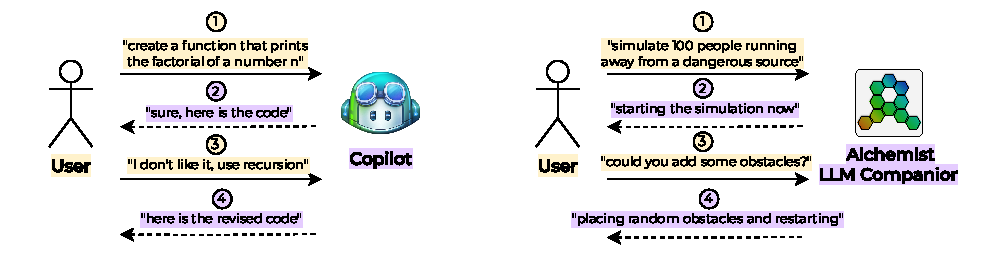
\includegraphics[width=2\columnwidth]{use-case}
    \caption{
        Comparison of the interaction between a user and copilot for code generation purposes (left),
        and a user and an \ac{LLM} companion for simulation purposes (right).
        %
        In the first case the user asks for assitance in generating code to solve a problem.
        The user does not like the generated code and asks for a new one, explaining what needs to be changed.
        %
        In the latter case the user wants to visualize a simulation scenario, and asks the \ac{LLM} the simulation scenario in natural language.
        Under the hood, the \ac{LLM} translates the natural language into a configuration file that can be used by the simulator and start a simulation for the user to monitor.
        %
        The user can then ask for changes,
        either because the simulation is not behaving as expected,
        or to explore the behavuiour in different scenarios.
    }
    \label{fig:usecase}
\end{figure*}

% Other things about LLM... to write
\section{Conclusion}
We have explored the complexities and challenges associated with designing effective and user-friendly \acp{HMI} for distributed general-purpose simulations.
%
The Alchemist simulator was used as a case study to illustrate some challenges and the potential solutions.
%
A transition from a desktop-based \ac{GUI} to a web-based \ac{GUI} has been proposed to overcome some limitations and increase the amount of support that external tools can provide.
%
However,
lots of research still needs to be conducted in order to improve the \ac{UX} of simulations.
%
\ac{LLM} and similar technologies are promising and pervasive tools that can be used to assist users in solving everyday problems,
and simulations are no exception.
%
There are several possible way to effectively design an \ac{LLM} in order to improve the prompts and get better results.
%
One example that could suite the simulation use case is the ReAct prompting technique~\cite{DBLP:conf/iclr/YaoZYDSN023},
which focuses on generating both reasoning traces and task-specific actions.
%
Moreover,
the framework is also able to retrieve information from external environments,
enabling to avoid fact hallucination.
%

\bibliographystyle{IEEEtran}
\bibliography{doctoral-colloquium-2024-dsrt-simulation-interaction}
\vspace{12pt}
\end{document}
